\documentclass[
  % Babel language, also used to load translations
  english,
  % Use A4 paper size, you can change this to eg. letterpaper if you need
  % the letter format. The normal methods to modify the paper size should
  % be picked up by SDAPS automatically.
  % a4paper, % setting this might break the example scan unfortunately
  % letterpaper
  %
  % If you need it, you can add a custom barcode at the center
  %globalid=SDAPS,
  %
  % And the following adds a per sheet barcode at the bottom left
  %print_questionnaire_id,
  %
  % You can choose between twoside and oneside. twoside is the default, and
  % requires the document to be printed and scanned in duplex mode.
  %oneside,
  %
  % With SDAPS 1.1.6 and newer you can choose the mode used when recognizing
  % checkboxes. valid modes are "checkcorrect" (default), "check" and
  % "fill".
  %checkmode=checkcorrect,
  ]{sdapsclassic}
\usepackage[utf8]{inputenc}
% For demonstration purposes
\usepackage{multicol}
\usepackage{graphicx}
\graphicspath{{coins/}}

\author{The Author}
\title{The Title}

\begin{document}
  % Everything you do should be done inside the questionnaire environment.

  % If you don't like the default text at the beginning of each questionnaire
  % you can remove it with the optional [noinfo] parameter for the environment 
  \begin{questionnaire}
    % There is a predefined "info" style to hilight some text.
    \begin{info}
      You can create a customized information element similar to the standard
      one using the \texttt{info} environment. By adding \texttt{[noinfo]} to
      the \texttt{questionaire} environment you can replace the predefined
      information field with your own.
    \end{info}

    % Use \addinfo to add metadata (which is printed on the report later on)
    \addinfo{Date}{10.03.2013}

    % You can structure the document using sections. You should not use
    % subsections yourself, as these are used to typeset question text.
    \section{Range Questions}

    % Lets ask some questions.
    % \singlemark creates a single range (1-5) question.
    \singlemark{How often do you use SDAPS?}{never}{daily}

    % Now we would like to ask multiple range questions that are similar. We
    % can use a markgroup environment to typeset many range questions under
    % one heading.
    \begin{markgroup}{What do you think about the following aspects of \LaTeX?}
      \markline{equation syntax}{bad}{good}
      \markline{rendered equations}{ugly}{beautiful}
      \markline{ease of use}{hard}{easy}
    \end{markgroup}

    \section{Choice Questions}
    We can also give users a question with predefined choices. Such a list
    of choices is typesetted using a tabularx environment with equally
    sized columns. Items can span multiple columns.

    \begin{choicequestion}[cols=3]{Which of the following Open Source
                                   Optical Mark Recognition software
                                   packages have you heard about?}
      \choiceitem{SDAPS}
      \choicemulticolitem{2}{Auto Multiple Choice}
      \choiceitem{QueXF}

      % Insert a text field. The freeform box automatically scales horizontally
      % The first parameter is the height of the box. The second parameter
      % is the amount of columns it should span.
      \choiceitemtext{1.2cm}{2}{Other:}
    \end{choicequestion}

    % And a more compact way of doing it; similar to markgroup
    \begin{choicegroup}{Which software do you prefere for the following tasks?}
      % We have to add the possible choices at the start.
      \groupaddchoice{\LaTeX}
      \groupaddchoice{LibreOffice}
      \groupaddchoice{Microsoft Word}
      \groupaddchoice{other}

      % After that it is possible to add each question.
      \choiceline{writing letters}
      \choiceline{creating tables}
      \choiceline{typesetting equations}
    \end{choicegroup}

    \section{Freeform text fields}

    SDAPS will extract freeform textfields such as below as images and put
    these into reports. SDAPS knows whether there is writing in the box and
    how large it is.

    % This is a textbox which is at least 2cm high. It will automatically scale
    % to fill the page.
    \textbox{2cm}{Do you have any comments?}

    % Force a new page here
    \newpage
    \section{Tricks and Features}
    You can use the {\ttfamily multicol} package to create multi-column layouts
    as is done below.

    \begin{multicols}{2}
      % We should use text= here to not get the label, but the class does not
      % yet support this.
      \singlemark{This is a range question\label{somelabel}}{lower bound}{upper bound}

      As you can see, this is a multi-column layout. The {\ttfamily markgroup} and
      {\ttfamily choicegroup} environments may be a bit tight in this mode.

      Lets put some more questions here, just because we can.

      \begin{choicequestion}[cols=1]{A choice question!}
        \choiceitem{first choice}
        \choiceitem{second choice}
        \choiceitem{third choice}
        \choiceitemtext{1.2cm}{1}{other:}
      \end{choicequestion}

      \singlemark{Another range question}{lower bound}{upper bound}
      This text is closer to the question compared to question~\ref{somelabel}
      because it is not starting a new paragraph.


      \textbox{3cm}{And a freeform text field}
    \end{multicols}

    That's it for the multi-column part; it was fun while it lasted!

    There are some more special commands. You can draw \checkedbox{} crossed
    checkboxes, \filledbox{} filled or \correctedbox{} filled and crossed ones. Finally there is
    also the plain \checkbox{} checkbox using {\ttfamily \textbackslash{}checkbox}
    or the starred versions showing single choice items \checkbox*{}
    \checkedbox*{}. These are for decoration purposes only and do not affect
    further processing in any way.

    \textbox*{2cm}{And textboxes with a fixed height. This one is exactly 2\,cm high.}

    \section{Images}

    If you intend to include images, it is a good idea to place them (and all other
    files you need) into a subdirectory. You can then use \texttt{sdaps setup --add DIR}
    to make sure the files are copied into the project.

    \begin{choicequestion}[cols=5]{Which of the following coins are from Indonesia?}
      \choiceitem[text=200 Indonesian Rupia]{
        \raisebox{-1.5em}{
          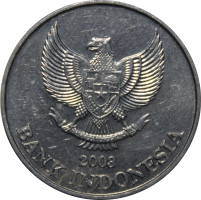
\includegraphics[height=4em,keepaspectratio]{coins/200_rupiah_coin_obverse.jpg}
        }
      }
      \choiceitem[text={Bactriane, Eucratide I, Back}]{
        \raisebox{-1.5em}{
          \includegraphics[height=4em,keepaspectratio]{coins/Eucratide_1er_-_20_stateres.jpg}
        }
      }
      \choiceitem[text=1000 Indonesian Rupia]{
        \raisebox{-1.5em}{
          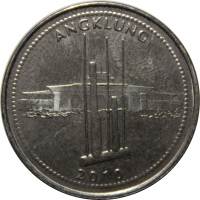
\includegraphics[height=4em,keepaspectratio]{coins/1000_rupiah_coin_reverse.jpg}
        }
      }
      \choiceitem[text={Aureus, Auguste, Lyon}]{
        \raisebox{-1.5em}{
          \includegraphics[height=4em,keepaspectratio,trim={0 0 200 0},clip]{coins/Aureus,_Auguste,_Lyon,_btv1b104440369.jpg}
        }
      }
      \choiceitem[text=Julius Caesar]{
        \raisebox{-1.5em}{
          \includegraphics[height=4em,keepaspectratio]{coins/RRC_452-2_Julius_Caesar_coin.jpg}
        }
      }
    \end{choicequestion}

    A nice way to make this more comfortable is to set an image search path.
    This example uses the command \verb^\graphicspath{{coins/}}^, so that the
    full path to the image is not needed each time. Note that you should not
    include a leading \texttt{./}.

     \begin{optiongroup}{}
       \choice[text={Aureus Auguste Lyon}]{\includegraphics[height=4em,keepaspectratio,trim={200 0 0 0},clip]{Aureus,_Auguste,_Lyon,_btv1b104440369.jpg}}
       \choice[text={Bactriane, Eucratide I}]{\includegraphics[height=4em,keepaspectratio]{Eucratide_1er_-_20_stateres.jpg}}
       \choice[text=Julius Caesar]{\includegraphics[height=4em]{RRC_452-2_Julius_Caesar_coin.jpg}}
       \question[text={Find the other side of Bactriane, Eucratide I, Face}]{Find the other side of \raisebox{-1.5em}{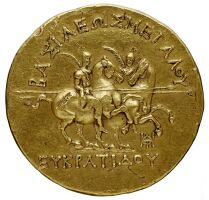
\includegraphics[height=4em,keepaspectratio]{Monnaie_de_Bactriane,_Eucratide_I,_face.jpg}}}
     \end{optiongroup}
  \end{questionnaire}
\end{document}

